\section{Results}

\subsection{Cohort and estimation sample}
The cohort comprised 6,627 first eligible mathematics-course attempts in 190 instructor--period clusters. The cluster-level split reserved 1,952 students from 57 clusters for validation and allocated 4,675 students from 133 clusters to discovery. In the eight-category visit grid, 5,393 students reported no visits, while the respective counts for exact one through six visits and seven or more were 517, 245, 170, 96, 55, 50 and 101. Both outcomes and both upper-tail representations completed 100 out of 100 cluster-bootstrap fits, with no recorded failures.

\subsection{Selected attendance regimes}
For instructor--period-standardised grades, the discovery-sample ordered fused lasso selected two blocks: $[0]$ and $[1,2,3,4,5,6,7+]$, using $\lambda=0.028091$. The same division emerged when exact six visits were pooled with the upper tail as $6+$. Among all 128 contiguous eight-category partitions, this two-block solution also had the most favourable discovery-sample relative BIC.

For PASS, the conservative one-standard-error-style cross-validation heuristic selected an all-fused single block at $\lambda=0.024082$. Importantly, the minimum grouped-CV loss occurred at $\lambda=0.000360$, with MSE 0.168915 versus 0.173192 for the selected all-fused model. The latter difference was permitted by the four-fold estimated tolerance, which is a parsimony heuristic rather than an inferential standard error. The discovery-only Gaussian-working-model BIC ranked the all-fused solution last of 128; its best-ranked alternative had cuts $0|1$ and $3|4$, followed by $0|1$ alone (relative BIC difference approximately 1.53). Neither ranking is a held-out hypothesis test, and changing the selection rule after observing these results would require explicitly labelled sensitivity analysis.

\subsection{Bootstrap boundary stability}
Table~\ref{tab:selection} reports selection frequencies from 100 successful whole-classroom bootstrap replicates, each repeating lambda selection. For standardised grades, the initial $0|1$ boundary was selected in every replicate, while no other positive-frequency boundary exceeded 10\%. For PASS, the same initial boundary appeared in only 37\% of replicates. Frequencies of selected cuts are neither $p$-values nor measures of equivalence within fused blocks.

\begin{table}[ht]
\centering
\caption{Frequency of selecting each primary-grid visit boundary in 100 cluster-bootstrap replicates.}
\label{tab:selection}
\begin{tabular}{lrr}
\toprule
Visit boundary & Standardised grade (\%) & PASS (\%)\\
\midrule
$0|1$ & 100 & 37\\
$1|2$ & 10 & 2\\
$2|3$ & 0 & 0\\
$3|4$ & 1 & 1\\
$4|5$ & 0 & 0\\
$5|6$ & 0 & 0\\
$6|7+$ & 0 & 0\\
\bottomrule
\end{tabular}
\end{table}

\IfFileExists{../../results/paper221/figures/7plus_z_grade_primary_boundary_stability.pdf}{
\begin{figure}[ht]
\centering
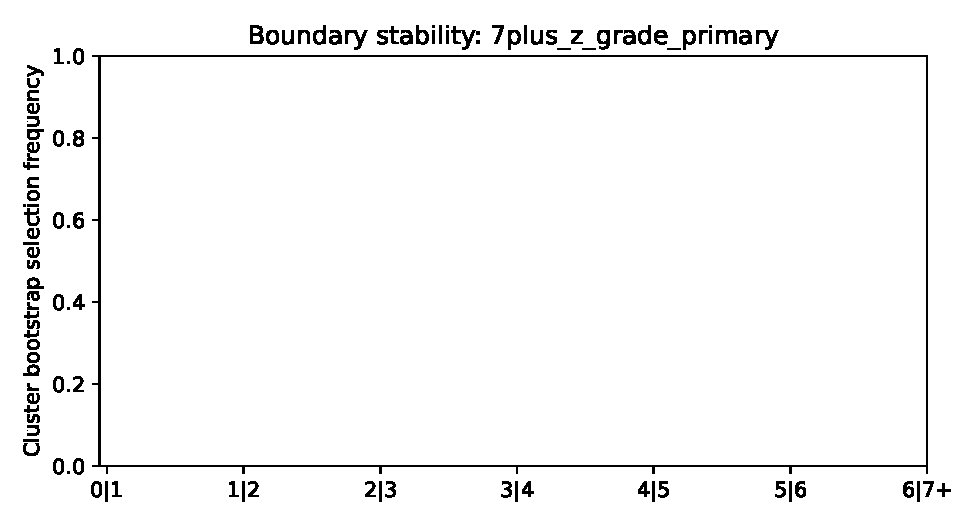
\includegraphics[width=.8\linewidth]{../../results/paper221/figures/7plus_z_grade_primary_boundary_stability.pdf}
\caption{Selection frequency of each adjacent cut for standardised grades. The penalisation is reselected in each discovery-classroom bootstrap sample.}
\end{figure}
}{}

\IfFileExists{../../results/paper221/figures/7plus_pass_boundary_stability.pdf}{
\begin{figure}[ht]
\centering
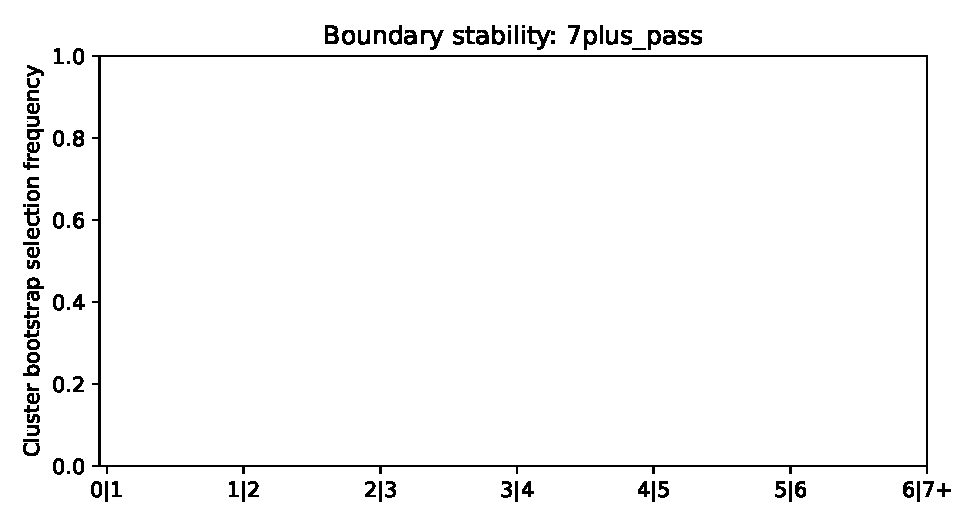
\includegraphics[width=.8\linewidth]{../../results/paper221/figures/7plus_pass_boundary_stability.pdf}
\caption{Corresponding bootstrap selection frequency for the PASS outcome; an all-fused model is a penalised representation, not an equivalence test.}
\end{figure}
}{}

\subsection{Reserved-cluster validation}
Refitting the two selected Z blocks without penalisation in the 57 reserved instructor--period clusters gave an adjusted difference of 0.2636 standard deviations between students with at least one visit and students with none (cluster-robust standard error 0.0580, nominal 95\% CI 0.150--0.377, Wald and Holm-adjusted $p=5.44\times10^{-6}$). Among 1,952 validation observations, 1,585 had zero visits and 367 had positive visits; 52 clusters contained both blocks. PASS selected no boundary and therefore has no corresponding selected-boundary Wald test. Its absence is not evidence of a zero effect.

The new fusion algorithm did not use validation outcomes for its tuning or bootstrap. Nevertheless, these observations belong to the wider cohort already examined in Paper 2.1, so this analysis offers \emph{internal algorithmic validation}, not a prospectively untouched or externally replicated confirmatory sample.

\subsection{Tail-pooling and pending sensitivities}
The pooled-$6+$ analysis reproduced the same grade and PASS partitions, with the $0|1$ boundary selected in 100\% and 37\% of bootstrap replicates, respectively. Numeric complete-case Z, instructor-level dependence, repeated grouped folds and a minimum-CV-loss penalty-selection sensitivity remain to be evaluated; the published estimates should not be described as robust to these unperformed analyses.
